% This is samplepaper.tex, a sample chapter demonstrating the
% LLNCS macro package for Springer Computer Science proceedings;
% Version 2.20 of 2017/10/04
%
\documentclass[runningheads]{llncs}
%
\usepackage{graphicx}
\usepackage{subfigure}
% Used for displaying a sample figure. If possible, figure files should
% be included in EPS format.
%
% If you use the hyperref package, please uncomment the following line
% to display URLs in blue roman font according to Springer's eBook style:
% \renewcommand\UrlFont{\color{blue}\rmfamily}

\begin{document}
%
\title{Programming Assignment 1 Solution}
\author{Fahim Tahmid Chowdhury}
\institute{Florida State University}
\maketitle              % typeset the header of the contribution
%

\section{Support Vector Machine (SVM)}
\subsection{Answer to 1(a)}
The soft margin classification algorithm is implemented in the \texttt{svm\_model.py} file of the submitted code.

\subsection{Answer to 1(b)}
The random dataset is generated according to the project specification while keeping the random seed fixed to 33290.
The dataset generation is implemented in \texttt{generate\_random\_data.py}.
The dataset is fed to the SVM model and the value of C is varied from 1000.1, 100.1, 0.001 to 0.0001.
\figurename~\ref{fig:svm_c_1000.1}, \figurename~\ref{fig:svm_c_100.1}, \figurename~\ref{fig:svm_c_0.001} and
\figurename~\ref{fig:svm_c_0.0001} depict the results for SVM model when C = 1000.1, 100.1, 0.001 and 0.0001, respectively.
All the figures show the datapoints, i.e. red crosses and green crosses belong to Class A and B respectively,
the support vectors are circles by blue circles. The classifier is denoted by the solid black line and the decision boundaries are shown by the dashed lines.
The misclassification error, leave-one-out cross validation error and margin for different values of C are mentioned in Table~\ref{tab:table_C}.
For the dummy dataset, we find that the misclassification and leave-one-out cross validation error are the same. With decreasing
value of the tradeoff variable, C, both the types of error values increase and the margin increases.

\begin{table}
\caption{SVM results on dummy dataset for different values of C}\label{tab:table_C}
\begin{tabular}{|l|l|l|l|}
\hline
C &  Misclassification Error & Leave-one-out Cross Validation Error & Margin\\
\hline
1000.1 & 0.0825 & 0.0825 & 0.4736146883359073\\
100.1 & 0.085 & 0.085 & 0.473277758987939\\
0.001 & 0.085 & 0.085 & 2.4963754697373535\\
0.0001 & 0.0875 & 0.0875 & 17.677670988643605\\
\hline
\end{tabular}
\end{table}

\begin{figure*}[h!]
    \vspace{-0.0pc}
    \begin{center}
       \subfigure[C=1000.1\label{fig:svm_c_1000.1}]
       {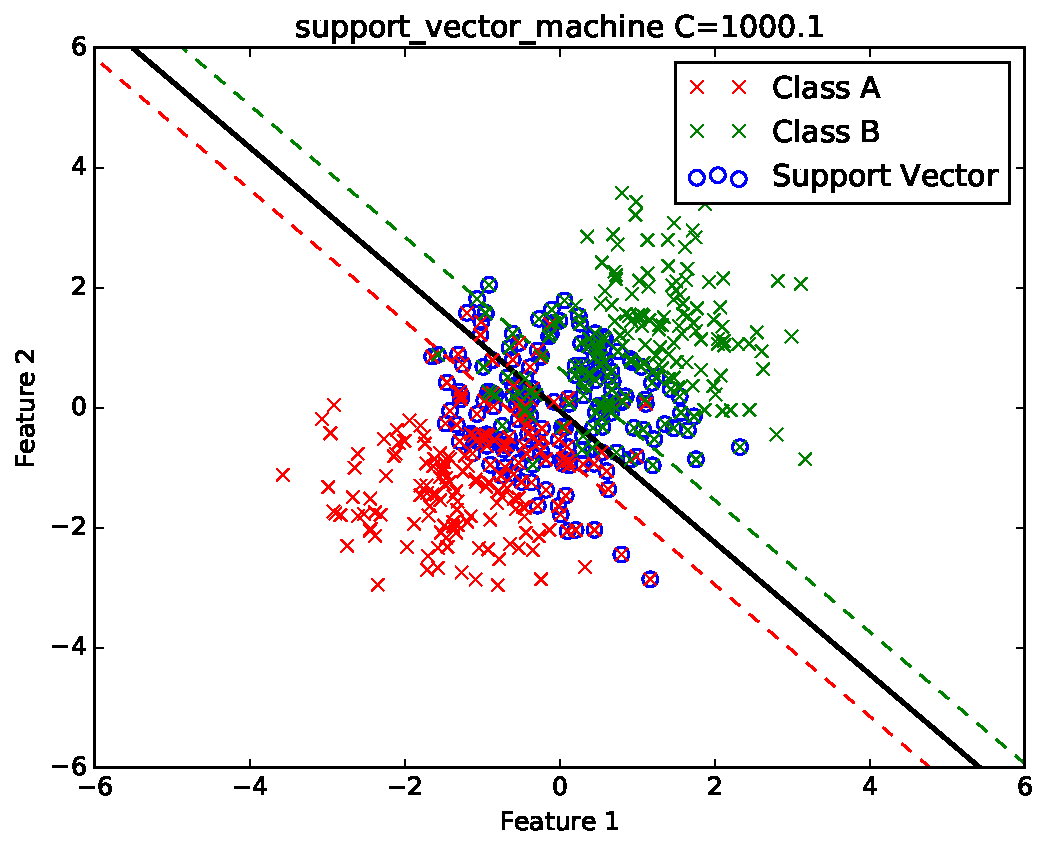
\includegraphics[width=0.49\textwidth]{support_vector_machine1000_1.pdf}}
       \subfigure[C=100.1\label{fig:svm_c_100.1}]
       {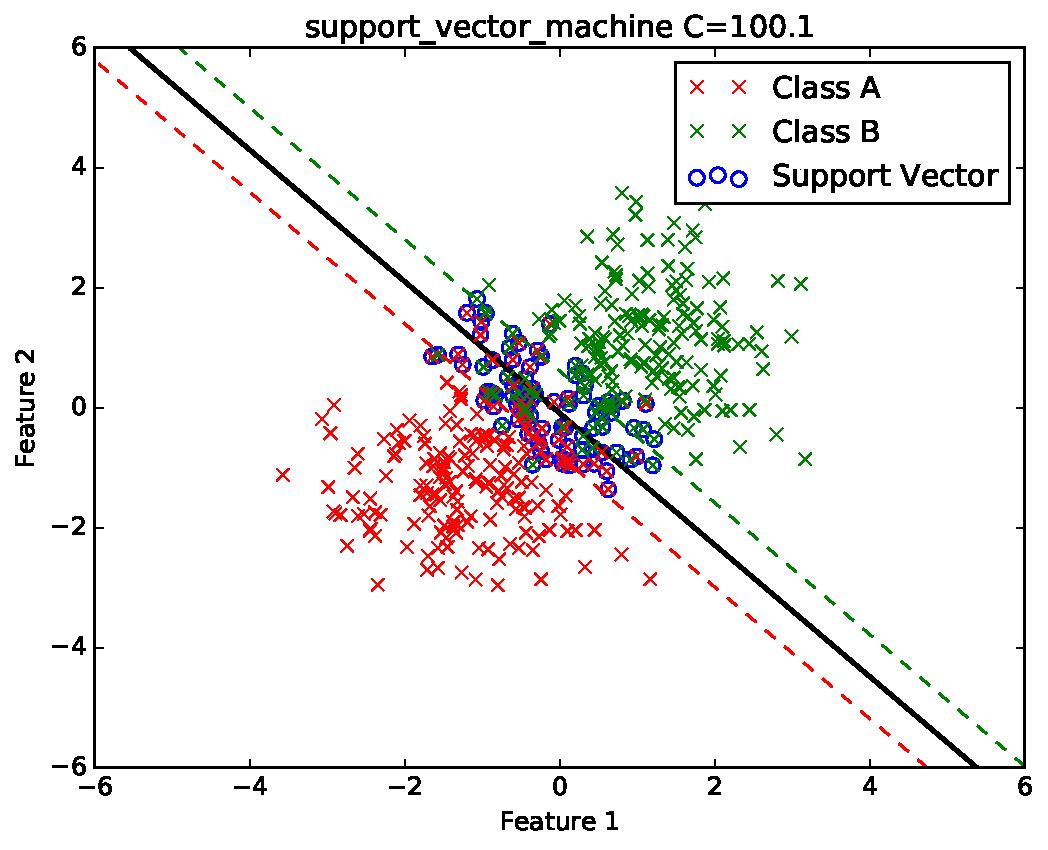
\includegraphics[width=0.49\textwidth]{support_vector_machine100_1.pdf}}
       \subfigure[C=0.001\label{fig:svm_c_0.001}]
       {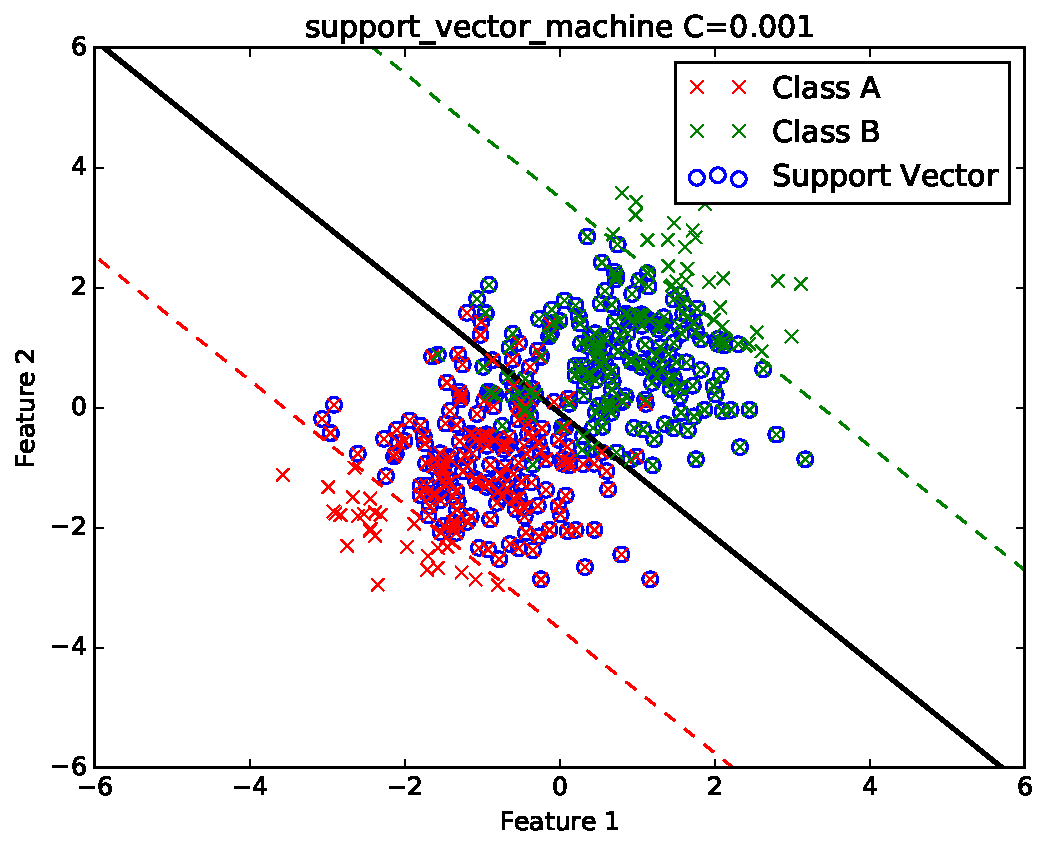
\includegraphics[width=0.49\textwidth]{support_vector_machine0_001.pdf}}
       \subfigure[C=0.0001\label{fig:svm_c_0.0001}]
       {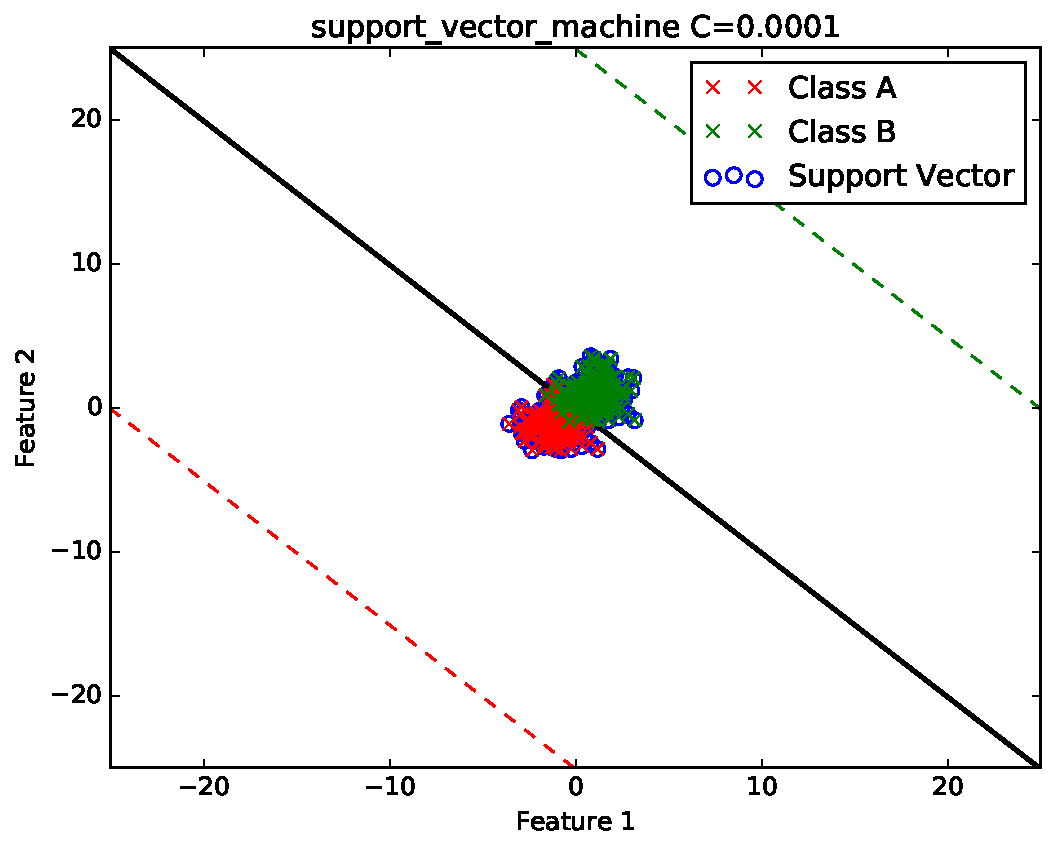
\includegraphics[width=0.49\textwidth]{support_vector_machine0_0001.pdf}}
       \vspace{-0.0pc}
       \caption{SVM model plots for variable C}
       \label{fig:svm}
    \end{center}
  \vspace{-1.0pc}
\end{figure*}

\subsection{Answer to 1(c)}
Only the samples with 0 and 1 labels in the MNIST dataset are filtered out in \texttt{mnist\_reader.py} file.
For training the SVM model with MNIST, the value for the tradeoff variable C is set to 1000.1.
The generalization error is 0.0009456264775413711 in this case.

\section{Regression}

\subsection{Answer to 2(a)}
The linear regression implementation is in \texttt{linear\_regression\_model.py} file. Here, the learning rate is
set to 0.001 and number of maximum iterations is kept as 10000. The binary classifier has a 0.0 threshold.
It returns +1 for Class A and -1 for Class B. \figurename~\ref{fig:linear_dummy} shows the decision boundary
of the classifier indicated by the solid black line. The training points are also plotted, i.e. red crosses are
Class A and green crosses are Class B training points. The leave-one-out cross validation error here is 0.085.
For convergence, the mean squared error is calculated for measuring the loss function. The maximum value
allowed here is $2^{300}$ for avoiding overflow issue in Python.
\begin{figure}
\centering
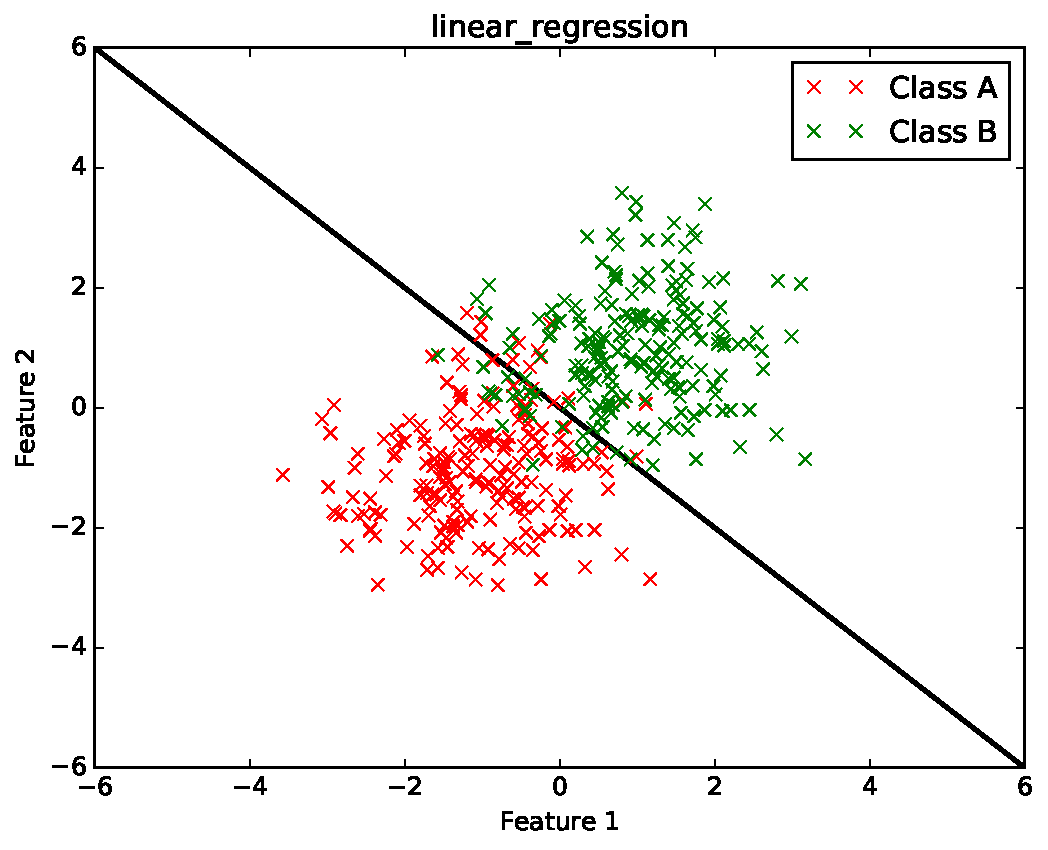
\includegraphics[width=0.75\textwidth]{linear_regression.pdf}
\caption{Linear regression on dummy dataset} \label{fig:linear_dummy}
\end{figure}

\begin{figure}
\centering
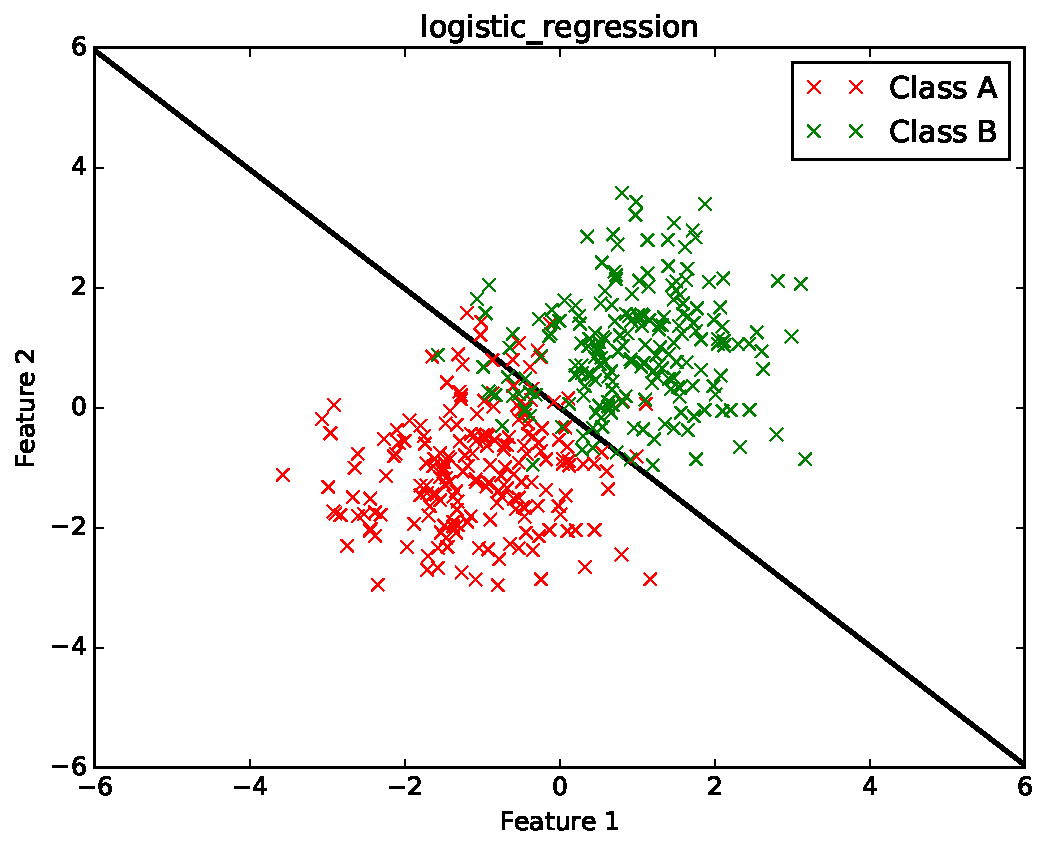
\includegraphics[width=0.75\textwidth]{logistic_regression.pdf}
\caption{Logistic regression on dummy dataset} \label{fig:logistic_dummy}
\end{figure}
\subsection{Answer to 2(b)}
The logistic regression implementation is in \texttt{logistic\_regression\_model.py} file. Here, the learning rate is
set to 0.001 and number of maximum iterations is kept as 10000. The binary classifier predicts +1 if the
sigmoidal function value is more than or equal to 0.5, otherwise it predicts -1.
As usual, it returns +1 for Class A and -1 for Class B. \figurename~\ref{fig:logistic_dummy} shows the decision boundary
of the classifier indicated by the solid black line. The training points are also plotted, i.e. red crosses are
Class A and green crosses are Class B training points. The leave-one-out cross validation error here is 0.085.
For convergence, cross entropy or log loss function is calculated for measuring the loss function. $1e^{-10}$ is
added to predicted value in the loss function to avoid division by zero exceptions in Python.

\subsection{Answer to 2(c)}
The comparison of the generalization errors of distinguishing between class 0 and class 1 on the MNIST
dataset is stated in Table~\ref{tab:comp}. According to the experimental results, the linear regression
classifier does not work well for MNIST dataset. Logistic regression classifier is a bit better, but not
up to the mark. On the other hand, the SVM model performs really well for MNIST.
\begin{table}
\centering
\caption{Generalization Errors Comparison}\label{tab:comp}
\begin{tabular}{|l|l|}
\hline
Model &  Generalization Error\\
\hline
Linear Regression & 0.5366430260047281\\
Logistic Regression & 0.2936170212765957\\
SVM & 0.0009456264775413711\\
\hline
\end{tabular}
\end{table}

\end{document}
